
% This LaTeX was auto-generated from MATLAB code.
% To make changes, update the MATLAB code and republish this document.

\documentclass{article}
\usepackage{graphicx}
\usepackage{color}

\sloppy
\definecolor{lightgray}{gray}{0.5}
\setlength{\parindent}{0pt}

\begin{document}

    
    

\section*{9. Gibbs phenomenon}

\begin{verbatim}
ATAPformats
\end{verbatim}
\begin{par}
Polynomial interpolants and projections oscillate and overshoot near discontinuities. We have observed this \textit{Gibbs phenomenon} already in Chapter 2, and now we shall look at it more carefully.  We shall see that the Gibbs effect for interpolants can be regarded as a consequence of the oscillating inverse-linear tails of Lagrange polynomials, i.e., interpolants of Kronecker delta functions.  Chapter 15 will show that these same tails, combined together in a different manner, are also the origin of Lebesgue constants of size $O(\log n)$, with implications throughout approximation theory.
\end{par} \vspace{1em}
\begin{par}
To start, let us consider the function \texttt{sign(x)}, which we interpolate in $n+1 = 10$ and 20 Chebyshev points. We take $n$ to be odd to avoid having a gridpoint at the middle of the step.
\end{par} \vspace{1em}
\begin{par}
 \vskip -2em 
\end{par} \vspace{1em}
\begin{verbatim}
x = chebfun('x'); f = sign(x);
subplot(1,2,1), hold off, plot(f,'k','jumpline','-k'), hold on, grid on
f9 = chebfun(f,10); plot(f9,'.-'); FS = 'fontsize';
title('Gibbs overshoot, n = 9',FS,9)
subplot(1,2,2), hold off, plot(f,'k','jumpline','-k'), hold on, grid on
f19 = chebfun(f,20); plot(f19,'.-')
title('Gibbs overshoot, n = 19',FS,9)
\end{verbatim}

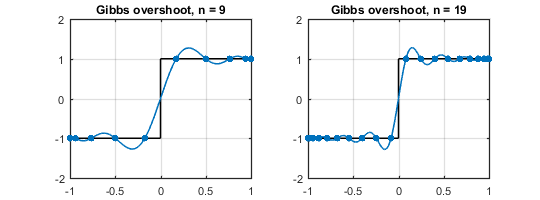
\includegraphics [width=4in]{chap9_01.png}
\begin{par}
 \vskip 1pt 
\end{par} \vspace{1em}
\begin{par}
Both of these figures show a substantial overshoot near the jump.  As $n$ increases from $9$ to $19$, the overshoot gets narrower, but not shorter, and it will not go away as $n\to\infty$. Let us zoom in and look at the plot on subintervals:
\end{par} \vspace{1em}
\begin{par}
 \vskip -2em 
\end{par} \vspace{1em}
\begin{verbatim}
subplot(1,2,1), hold off, plot(f,'k','jumpline','-k'), hold on, grid on
plot(f9,'.-','interval',[0 0.8]), axis([-.2 .8 .5 1.5])
title('Gibbs overshoot, n = 9',FS,9)
subplot(1,2,2), hold off, plot(f,'k','jumpline','-k'), hold on, grid on
plot(f19,'.-','interval',[0 0.4]), axis([-.1 .4 .5 1.5])
title('Gibbs overshoot, n = 19',FS,9)
\end{verbatim}

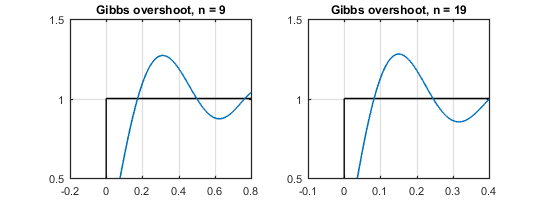
\includegraphics [width=4in]{chap9_02.png}
\begin{par}
 \vskip 1pt 
\end{par} \vspace{1em}
\begin{par}
We now zoom in further with analogous plots for $n=99$ and 999.
\end{par} \vspace{1em}
\begin{par}
 \vskip -2em 
\end{par} \vspace{1em}
\begin{verbatim}
subplot(1,2,1), hold off, plot(f,'k','jumpline','-k'), hold on
f99 = chebfun(f,100); plot(f99,'.-','interval',[0 0.08])
title('Gibbs overshoot, n = 99',FS,9)
grid on, axis([-.02 .08 .5 1.5])
subplot(1,2,2), hold off, plot(f,'k','jumpline','-k'), hold on
f999 = chebfun(f,1000); plot(f999,'.-','interval',[0 0.008])
set(gca,'xtick',-.002:.002:.01)
set(gca,'xticklabel',{'-0.002','0','0.002','0.004','0.006','0.008'})
title('Gibbs overshoot, n = 999',FS,9)
grid on, axis([-.002 .008 .5 1.5])
\end{verbatim}

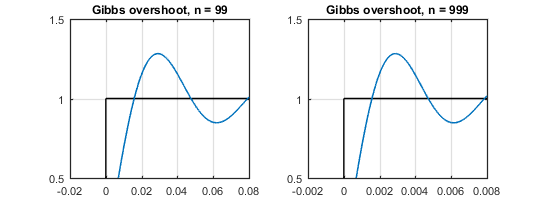
\includegraphics [width=4in]{chap9_03.png}
\begin{par}
 \vskip 1pt 
\end{par} \vspace{1em}
\begin{par}
Notice that in these figures, the vertical scale is always fixed while the horizontal scale is adjusted proportionally, confirming that the Gibbs overshoot gets narrower but approaches a constant height in the limit $n\to\infty$.
\end{par} \vspace{1em}
\begin{par}
What is this height?  We can measure it numerically with the \texttt{max} command:
\end{par} \vspace{1em}
\begin{par}
 \vskip -2em 
\end{par} \vspace{1em}
\begin{verbatim}
disp('     n        Gibbs amplitude')
for n = 2.^(1:8)-1
   gibbs = max(chebfun(f,n+1));
   fprintf('%7d  %17.8f\n', n, gibbs)
end
\end{verbatim}

        \color{lightgray} \begin{verbatim}     n        Gibbs amplitude
      1         1.00000000
      3         1.18807518
      7         1.26355125
     15         1.27816423
     31         1.28131717
     63         1.28204939
    127         1.28222585
    255         1.28226917
\end{verbatim} \color{black}
    \begin{par}
Clearly as $n\to\infty$, the maximum of the Chebyshev interpolant to the sign function converges to a number bigger than 1. The total variation of the interpolant, meanwhile, diverges slowly to $\infty$, at a rate proportional to $\log n$, and this is the effect we shall examine further in Chapter 15.
\end{par} \vspace{1em}
\begin{par}
 \vskip -2em 
\end{par} \vspace{1em}
\begin{verbatim}
disp('     n          variation')
for n = 2.^(1:8)-1
   tv = norm(diff(chebfun(f,n+1)),1);
   fprintf('%7d  %14.2f\n', n, tv)
end
\end{verbatim}

        \color{lightgray} \begin{verbatim}     n          variation
      1            2.00
      3            2.75
      7            3.64
     15            4.56
     31            5.47
     63            6.37
    127            7.26
    255            8.15
\end{verbatim} \color{black}
    \begin{par}
The following theorem summarizes the Gibbs phenomenon for Chebyshev interpolants.  Well, perhaps it is a little bold to call it a ``theorem'', since it is not clear that a proof has ever been written down.  The formulas necessary to represent the interpolant (in the equivalent trigonometric case---see Exercise 9.4) can be found in various forms in [Runck 1962] and [Helmberg \& Wagner 1997], which relates the interpolating polynomial to the beta function and reports the numbers $1.282$ and $1.066$ to three digits of accuracy. The more precise results presented here have been privately communicated to me by Wagner based on calculations to more than 500 digits.
\end{par} \vspace{1em}
\begin{par}
 \em
{\bf Theorem 9.1.  Gibbs phenomenon for Chebyshev interpolants.}
Let $p_n$ be the degree $n$ Chebyshev
interpolant of the function $f(x) = \hbox{\rm sign}(x)$ on $[-1,1]$.
Then as $n\to\infty$,
$$ \lim_{n\to\infty,\, n\,\hbox{\footnotesize odd}} \|\kern 1pt p_n\|
\,=\, c_1 \,=\, 1.28228345577542854813\dots, \eqno (9.1) $$
$$ \lim_{n\to\infty,\, n\,\hbox{\footnotesize even}} \|\kern 1pt p_n\|
\,=\, c_2 \,=\, 1.06578388826644809905\dots. \eqno (9.2) $$
(The case of $\kern 2pt n$ even differs in having a gridpoint at the middle
of the jump.)

\end{par} \vspace{1em}
\begin{par}

Although we are not going to prove Theorem 9.1, we do want to indicate
where the fixed-overshoot effect comes from.  Everything falls into place
when we consider the Lagrange polynomials introduced in Chapter 5.
Recall from (5.2) that the $j$th Lagrange polynomial $\ell_j(x)$ for the
$(n+1)$-point Chebyshev grid is the unique polynomial in ${\cal P}_n$
that takes the values $1$ at $x_j$ and $0$ at the other grid points
$x_k$. On the $20$-point grid, $\hbox{i.e.\ } n=19$,  here are the
Lagrange polynomials $\ell_{10}$ and $\ell_{11}$ with a dashed line
marked at $x=-0.15$, which we will take as our point of special interest.

\end{par} \vspace{1em}
\begin{par}
 \vskip -2em 
\end{par} \vspace{1em}
\begin{verbatim}
clf, yl = [-0.3 1.3];
xc = -0.15*[1 1];
p10 = chebfun([zeros(1,10) 1 zeros(1,9)]');
p11 = chebfun([zeros(1,11) 1 zeros(1,8)]');
subplot(1,2,1), plot(p10,'.-')
hold on, plot(xc,yl,'--r'), ylim(yl)
title('Lagrange polynomial  l_{10}',FS,9)
subplot(1,2,2), plot(p11,'.-')
hold on, plot(xc,yl,'--r'), ylim(yl)
title('Lagrange polynomial  l_{11}',FS,9)
\end{verbatim}

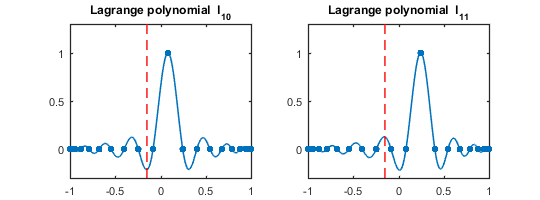
\includegraphics [width=4in]{chap9_04.png}
\begin{par}
 \vskip 1pt 
\end{par} \vspace{1em}
\begin{par}
Here are $\ell_{12}$ and $\ell_{13}$:
\end{par} \vspace{1em}
\begin{par}
 \vskip -2em 
\end{par} \vspace{1em}
\begin{verbatim}
p12 = chebfun([zeros(1,12) 1 zeros(1,7)]');
p13 = chebfun([zeros(1,13) 1 zeros(1,6)]');
subplot(1,2,1), hold off, plot(p12,'.-')
hold on, plot(xc,yl,'--r'), ylim(yl)
title('Lagrange polynomial  l_{12}',FS,9)
subplot(1,2,2), hold off, plot(p13,'.-')
hold on, plot(xc,yl,'--r'), ylim(yl)
title('Lagrange polynomial  l_{13}',FS,9)
\end{verbatim}

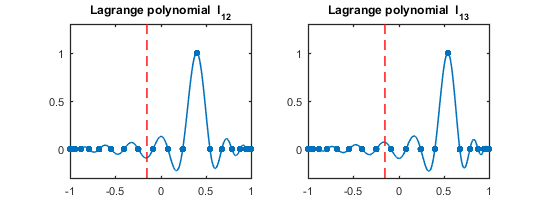
\includegraphics [width=4in]{chap9_05.png}
\begin{par}
 \vskip 1pt 
\end{par} \vspace{1em}
\begin{par}
Following (5.1), we note that by taking the sum of a sequence of such Lagrange functions, we get the interpolant to the function that jumps from 0 for $x<0$ to $1$ for $x>0$. Here is the sum of the four just plotted, which is beginning to look like a square wave:
\end{par} \vspace{1em}
\begin{par}
 \vskip -2em 
\end{par} \vspace{1em}
\begin{verbatim}
clf, plot(p10+p11+p12+p13,'.-')
hold on, plot(xc,yl,'--r'), ylim(yl)
title('l_{10} + l_{11} + l_{12} + l_{13}',FS,9)
\end{verbatim}

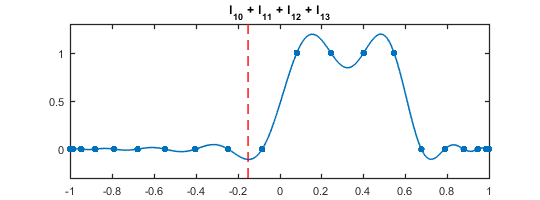
\includegraphics [width=4in]{chap9_06.png}
\begin{par}
 \vskip 1pt 
\end{par} \vspace{1em}
\begin{par}
If we went all the way to the last grid point we would get the interpolant $$ p(x) = \sum_{j = (n+1)/2}^n \ell_j(x).  $$ Note that for any fixed $x<x_{(n-1)/2}$, this is an \textit{alternating series} of small terms whose amplitudes decrease inverse-linearly to zero. The finite but nonzero sum of such a series in the limit $n\to\infty$ is what gives rise to the fixed overshoot Gibbs effect in polynomial interpolation.
\end{par} \vspace{1em}
\begin{par}
In particular, suppose we focus on the dashed line at $x=-0.15$ in the figures.  Notice the alternating signs of the values of $\ell_{10}, \ell_{11}, \ell_{12}, \ell_{13}$ at this value of $x$. In the figure for $\ell_{10}+\ell_{11}+\ell_{12}+\ell_{13}$ we accordingly see the Gibbs overshoot beginning to converge to its asymptotic amplitude $\approx 0.141$.  This number is half of the value $0.282\dots$ of Theorem 9.1, since the jump for this function is of amplitude 1 instead of 2.
\end{par} \vspace{1em}
\begin{par}
In Chapter 15 we shall consider the same alternating series but with signs multiplied by $(-1)^j$.  This eliminates the alternation, so that we have approximately a harmonic series of inverse-linear terms.  The partial sums of such a series grow at a logarithmic rate, as we saw above in the calculation of the variation.
\end{par} \vspace{1em}
\begin{par}

Our discussion so far has concerned interpolants, but there is a parallel
theory of the Gibbs phenomenon for projections---in the notation of this
book, polynomials $f_n$ rather than $p_n$. (The required Chebyshev
coefficients are defined by the same integral (3.12) of Theorem 3.1, even
though we are now dealing with functions $f$ that are not Lipschitz
continuous as in the assumption stated for that theorem.) As always,
though the interpolants are closer to practical computation, the
projections may appear to be more fundamental mathematically.
Historically speaking, it was the case of Fourier (trigonometric)
projection that was analyzed first. The original discoverer was not Gibbs
but Henry Wilbraham, a 22-year-old fellow of Trinity College, Cambridge,
in 1848, who unfortunately made the mistake of publishing his fine paper
in the short-lived {\em Cambridge and Dublin Journal of Mathematics}
[Wilbraham 1848]. Fourier series for certain functions with jumps were
already long known in Wilbraham's day---in fact they go back to Euler,
half a century before Fourier.  The particular series studied by
Wilbraham, originally due to Euler in 1772, is
$$ \cos(t) - {1\over 3} \cos (3t) + {1\over 5} \cos(5t) - \cdots,
\eqno (9.3) $$
which approximates a square wave of height $\pm \pi/4$ (compare
Exercise 3.6(a)):

\end{par} \vspace{1em}
\begin{par}
 \vskip -2em 
\end{par} \vspace{1em}
\begin{verbatim}
t = chebfun('t',[-6,6]);
f = (pi/4)*sign(cos(t));
clf, plot(f,'k','jumpline','k')
f9 = cos(t) - cos(3*t)/3 + cos(5*t)/5 - cos(7*t)/7 + cos(9*t)/9;
hold on, plot(f9), xlim([-6 6])
title('Partial sum of a Fourier series',FS,9)
\end{verbatim}

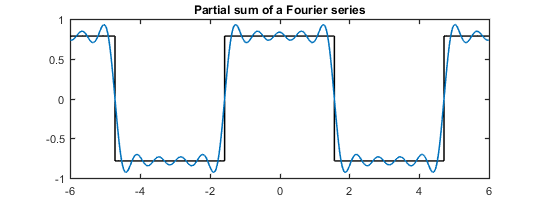
\includegraphics [width=4in]{chap9_07.png}
\begin{par}
 \vskip 1pt 
\end{par} \vspace{1em}
\begin{par}
Wilbraham worked out the magnitude of the overshoot, and thus the following analogue of Theorem 9.1 is due to him.
\end{par} \vspace{1em}
\begin{par}
 \em
{\bf Theorem 9.2.  Gibbs phenomenon for Chebyshev projections.}
Let $f_n$ be the degree $n$ Chebyshev projection of the sign function
$f(x) = \hbox{\rm sign}(x)$ on $[-1,1]$. Then as $n\to\infty$,
$$ \lim_{n\to\infty} \|f_n\| \,=\,
{2\over \pi} \int_0^\pi {\sin x\over x}\, dx \,=\,
1.178979744472167\dots . \eqno (9.4) $$
\vspace{-1.5em} 
\end{par} \vspace{1em}
\begin{par}
(The function $\hbox{Si}(x) = \int_0^x t^{-1}\sin t \kern 1pt dt$ is known as the \textit{sine integral}; see Exercise 9.6.) To see this number experimentally we can use the \texttt{'trunc'} option in the Chebfun constructor. The overshoots look similar to what we saw before, but with smaller amplitude.
\end{par} \vspace{1em}
\begin{par}
 \vskip -2em 
\end{par} \vspace{1em}
\begin{verbatim}
f = sign(x);
warnState = warning('off', 'CHEBFUN:constructor')
subplot(1,2,1), hold off, plot(f,'k','jumpline','k'), hold on, grid on
f9 = chebfun(f,'trunc',10); plot(f9,'-')
title('Gibbs projection overshoot, n = 9',FS,9)
subplot(1,2,2), hold off, plot(f,'k','jumpline','k'), hold on, grid on
f19 = chebfun(f,'trunc',20); plot(f19,'-')
title('Gibbs projection overshoot, n = 19',FS,9);
\end{verbatim}

        \color{lightgray} \begin{verbatim}warnState = 
    identifier: 'CHEBFUN:constructor'
         state: 'off'
\end{verbatim} \color{black}
    
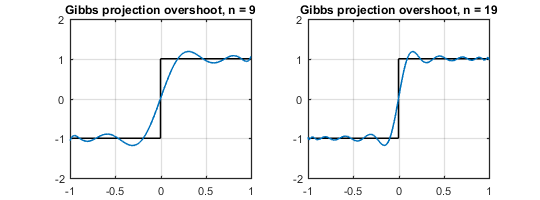
\includegraphics [width=4in]{chap9_08.png}
\begin{par}
 \vskip 1pt 
\end{par} \vspace{1em}
\begin{par}
The numbers behave as predicted:
\end{par} \vspace{1em}
\begin{par}
 \vskip -2em 
\end{par} \vspace{1em}
\begin{verbatim}
disp('     n       Gibbs amplitude')
for np = 2.^(4:7)
  g = chebfun(f,'trunc',np);
  fprintf('%7d  %17.8f\n', np, max(g{0,5/np}))
end
limit = (2/pi)*sum(chebfun('sin(x)./x',[0 pi]))
warning(warnState)
\end{verbatim}

        \color{lightgray} \begin{verbatim}     n       Gibbs amplitude
     16         1.18028413
     32         1.17930541
     64         1.17906113
    128         1.17900009
limit =
   1.178979744472168
\end{verbatim} \color{black}
    \begin{par}
In all the experiments of this chapter we have worked with polynomials rather than trigonometric series, but the effects are the same (Exercise 9.4).
\end{par} \vspace{1em}
\begin{par}
It is worth commenting on a particular property of series such as (9.3) that we have taken for granted throughout this discussion: even though each partial sum is continuous, a series may converge pointwise to a discontinuous limit, everywhere except at the points of discontinuity themselves.  This kind of behavior seems familiar enough nowadays, but in the century beginning with Fourier's work in 1807, it often seemed paradoxical and confusing to mathematicians.  The same pointwise convergence to discontinuous functions can also occur with interpolants, as in Theorem 9.1.
\end{par} \vspace{1em}
\begin{par}
In this chapter we have focussed on the height of the overshoot of a Gibbs oscillation, because this is the effect so readily seen in plots. Perhaps the most important property of Gibbs oscillations for practical applications, however, is not their height but their slow decay as one moves away from the point of discontinuity.  If $f$ has a jump, the oscillations at a distance $k$ gridpoints away must be expected to be of size $O(k^{-1})$; if $f'$ has a jump we expect oscillations of size $O(k^{-2})$, and so on.  (Exercise 26.5 will look at the analogous exponents for interpolation by rational functions rather than polynomials.)  This algebraic rate of decay of information in polynomial interpolants can be contrasted with the exponential decay that one gets with spline approximations, which is the key advantage of splines for certain applications. Chebfun responds to this problem by representing functions with discontinuities by piecewise polynomials rather than global ones, with breakpoints at the discontinuities. For example, the location of the discontinuity in the function $\exp(|x-0.1|)$ will be determined automatically in response to the command
\end{par} \vspace{1em}
\begin{par}
 \vskip -2em 
\end{par} \vspace{1em}
\begin{verbatim}
f = chebfun(@(x) exp(abs(x-0.1)),'splitting','on');
\end{verbatim}
\begin{par}
The result is a chebfun consisting of two pieces each of degree 3, and the break in the middle appears at the right place:
\end{par} \vspace{1em}
\begin{par}
 \vskip -2em 
\end{par} \vspace{1em}
\begin{verbatim}
f.ends(2)
\end{verbatim}

        \color{lightgray} \begin{verbatim}ans =
   0.100000000000000
\end{verbatim} \color{black}
    \begin{par}
Let us return to 22-year-old $\hbox{Mr.}$ Wilbraham.  Unfortunately, his published paper had little impact, and the effect was rediscovered and discussed in the pages of \textit{Nature} during 1898--1899 by James Michelson, A. E. H. Love, and J. Willard Gibbs. These authors got more attention for a number of reasons. First, they were leading scientists.  Second, their problem arose at a time when applied mathematics had advanced much further and in a practical application (a mechanical graphing machine called a ``harmonic analyser'' used by Michelson and Stratton).  Third, they published their observations in a major journal.  Fourth, they failed to get it right at first, so several publications appeared in succession!  Other mathematicians got involved too, notably $\hbox{Poincar\'e}$. Finally, they were lucky enough to have ``Gibbs's phenomenon'' named and highlighted a few years later in a major research article on Fourier analysis by the mathematician Maxime $\hbox{B\^ocher}$ [1906]. For a fascinating discussion of the history of the Gibbs phenomenon (for projection, not interpolation), which they more properly call the \textit{Gibbs--Wilbraham phenomenon}, see [Hewitt \& Hewitt 1979].
\end{par} \vspace{1em}
\begin{par}

\begin{displaymath}
\framebox[4.7in][c]{\parbox{4.5in}{\vspace{2pt}\sl
{\sc Summary of Chapter 9.}
Chebyshev projections and interpolants, as well as other polynomial and
trigonometric approximations, tend to oscillate near discontinuities.
The oscillations decay algebraically, not exponentially, with distance
from the discontinuity.
\vspace{2pt}}}
\end{displaymath}

\end{par} \vspace{1em}
\begin{par}
 \small\smallskip\parskip=2pt
{\bf Exercise 9.1.  \boldmath Calculations for larger $n$.}
We measured the height of the Gibbs overshoot for a step function for $n
= 1,3,7,\dots, 255$. Larger values of $n$ get a bit slow, but knowing
that the maximum occurs around $x = 3/n$, compute these numbers up to
$n=4095$ using a command of the form \verb|max(g{0,5/n})|.  How great a
speedup does this trick produce?
\par
{\bf Exercise 9.2.  A function with many jumps.}  Use Chebfun to produce
a plot of the degree 200 Chebyshev interpolant to the
function \verb|round(exp(sin(2*pi*x)))| on $[-1,1]$.
\par
{\bf Exercise 9.3.  Lagrange polynomials.}  Take $n\ge 2$ to be even and
let $p$ be the degree $n$ Chebyshev interpolant to the Kronecker delta
function at $x = x_{n/2} = 0$.  (a) Use the barycentric formula of
Theorem 5.2 to obtain a simple formula for $p$. (b) Derive a formula for
the values of $p$ at the ``Chebyshev midpoints'' defined by the usual
formula $x_j = \cos(\kern .7pt j\pi/n)$ of Chapter 2 except with
half-integer values of $j$.  (c) For $n=100$, use Chebfun to produce an
elegant plot showing the inverse-linear amplitudes of these values.  (You
can get the Chebyshev midpoints from \verb|chebpts(n,1)| or from
\verb|x=chebpts(2*n+1)|, \verb|x=x(2:2:end)|.)
\par
{\bf Exercise 9.4.  Fourier and Chebyshev Gibbs phenomena.} We have
repeatedly made the connection between Chebyshev polynomials $T_n(x)$ on
the unit interval, Laurent polynomials $(z^n+z^{-n})/2$ on the unit
circle, and trigonometric polynomials $\cos(n\theta)$ on $[-\pi,\pi]$.
Use these connections to show that the Gibbs overshoot in Chebyshev
interpolation of $\hbox{sign}(x)$ on $[-1,1]$, with $n$ even, is
identical to the overshoot for a certain problem of trigonometric
interpolation in $\theta$.
\par
{\bf Exercise 9.5.  Local minima of a truncated sine series.}
(a) Plot $\phi_n$ with $n = 10,100,$ and $1000$ for a sum going back
to Euler in 1755,
$$ \phi_n(x) = \sum_{k=1}^n {\sin(kx)\over k}. $$
What function does the sum evidently converge to?
Is the Gibbs overshoot of the same relative magnitude as for
(9.3)?
(b) For each case, determine the first four local minimum values of
$\phi_n(x)$ in $(0,\pi)$.  (c) Write an elegant Chebfun program that
determines the smallest value of $n$ for
which these minima are not monotonically decreasing.
(This effect was investigated by Gronwall [1912].)
\par
{\bf Exercise 9.6.  Sine integral.}
(a) Construct and plot a chebfun for the sine integral
$\hbox{Si}(x) = \int_0^x t^{-1} \sin t$ for $x\in[0,10]$.
What is its length?  (b) Same for $x\in[0,100]$.
(c) Same for $x\in[0,1000]$.
\par
{\bf Exercise 9.7.  An unresolvable function.}
The command \verb|f = chebfun(| \verb|'sin(1./x)',100000)| produces a
polynomial interpolant to $\sin(1/x)$ through 100,000 Chebyshev points.
The plot produced by \verb|plot(f)| looks as if there is a bug in the
computation somewhere.  Produce similar plots for 10000, 1000, and
smaller even numbers of points and explain why in fact, there is no bug.
\par
{\bf Exercise 9.8.  Decay away from discontinuity.} Plot the function
$f(x) = \cos(7x)\sin(3x) + \hbox{sign}(\sin(x/2))e^x$ on $[-1,1]$ as well
as its interpolating polynomial $p_n(x)$ in $n+1=100$ Chebyshev points.
Confirm the algebraic rate of decay away from the discontinuity by
plotting $|f(x)-p_n(x)|$ together with the function $c/|x|$ for a
suitable value of $c$.
\par

\end{par} \vspace{1em}



\end{document}
    
